\documentclass[sumlimits, intlimits]{beamer}

\usepackage[utf8]{inputenc}
\usepackage[T1]{fontenc}
\usepackage[english]{babel}
\usepackage{hyperref}
\usepackage{lmodern, microtype}
\usepackage[margin=2cm]{caption}
\usepackage{booktabs}
\usepackage{graphicx}

\usepackage{amsfonts, amsmath, amssymb}
\usepackage{mathtools}
\newcommand \twopi{{{\scriptstyle(2}\mskip-2.0mu\pi{\scriptstyle)}}}
\newcommand \ee{{\mathrm e}}
\newcommand \ii{{\mathrm i}}
\newcommand \full{{\mathrm d}}
\newcommand \fulld[1]{{\frac \full{\full {#1}}}}
\newcommand \partiald[1]{{\frac \partial{\partial {#1}}}}
\newcommand \yesnumber{\addtocounter{equation}{1}\tag \theequation}

\usepackage{listings}
\lstset{basicstyle=\footnotesize\ttfamily, tabsize=2}

\usepackage[backend=bibtex]{biblatex}
\addbibresource{refs.bib}

\title{ECMI Modelling Week 2018}
\subtitle{Storing Your Random Objects}
\author[shortname]{Desiré Nilsson \inst 1 \and
Ivana Gengeljacki \inst 5 \and
Jacob Hansen \inst 3 \and
Kirill Kiselev \inst 2 \and
Monika Žunji \inst 5 \and
Sampsa Kiiskinen \inst 4}
\institute[shortinst]{
\inst 1 Lund University \and
\inst 2 Saint Petersburg Polytechnic University \and
\inst 3 Technical University of Denmark \and
\inst 4 University of Jyväskylä \and
\inst 5 University of Novi Sad}
\date{2018-07-15 -- 2018-07-21}

\beamertemplatenavigationsymbolsempty

\usecolortheme{dove}
\usecolortheme{rose}
\usecolortheme{seahorse}

\mode<presentation>

\begin{document}

\begin{frame}
\titlepage
\end{frame}

\begin{frame}
\frametitle{Introduction}
\begin{block}{Filler Content}
Some literature \cite{conway-1998} goes here.
\end{block}
\end{frame}

\begin{frame}
\frametitle{Bottom-to-Top Reconstruction}
\begin{block}{Sketch of the Algorithm}
\centering
\def \h{7cm}
\only<1>{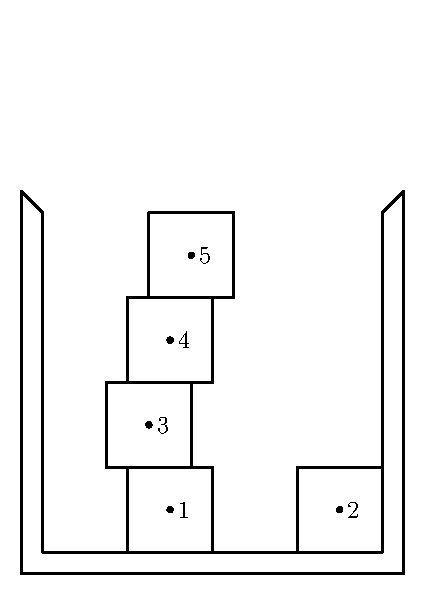
\includegraphics[height=\h]{btr-0}}%
\only<2>{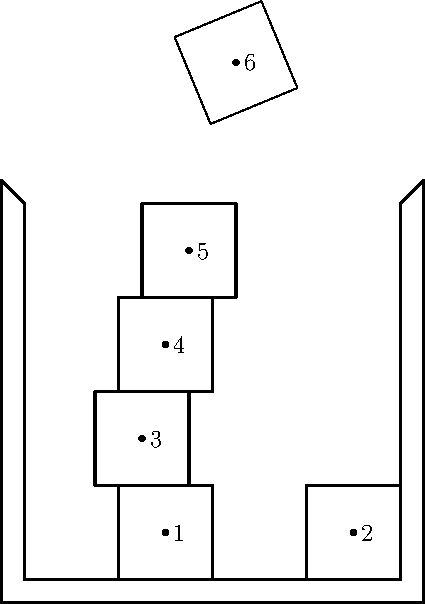
\includegraphics[height=\h]{btr-1}}%
\only<3>{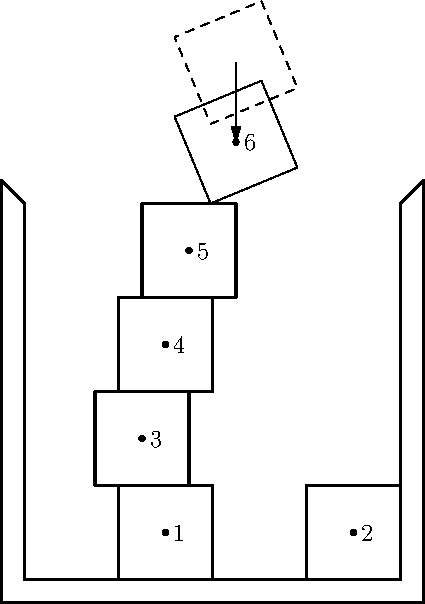
\includegraphics[height=\h]{btr-2}}%
\only<4>{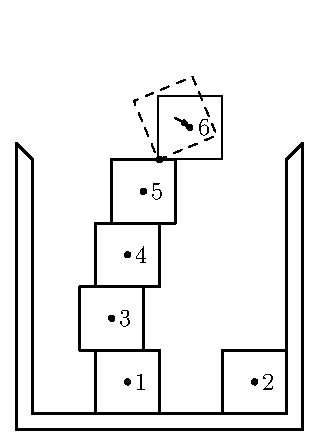
\includegraphics[height=\h]{btr-3}}%
\only<5>{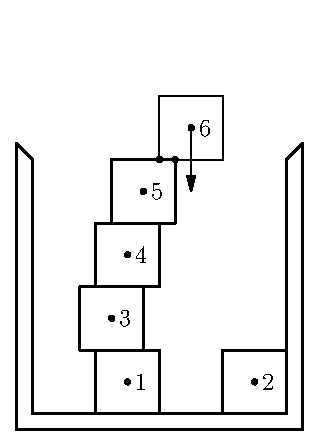
\includegraphics[height=\h]{btr-4}}%
\only<6>{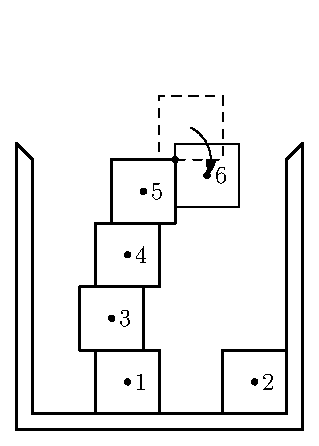
\includegraphics[height=\h]{btr-5}}%
\only<7>{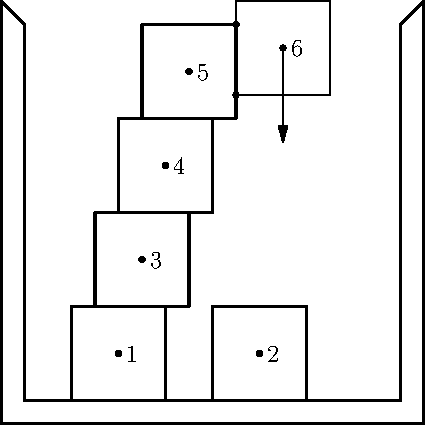
\includegraphics[height=\h]{btr-6}}%
\only<8>{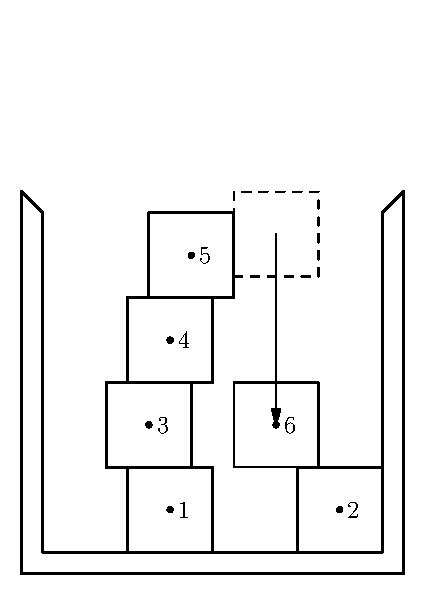
\includegraphics[height=\h]{btr-7}}%
\only<9>{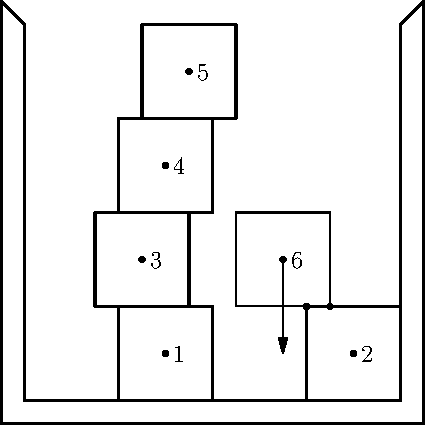
\includegraphics[height=\h]{btr-8}}%
\only<10>{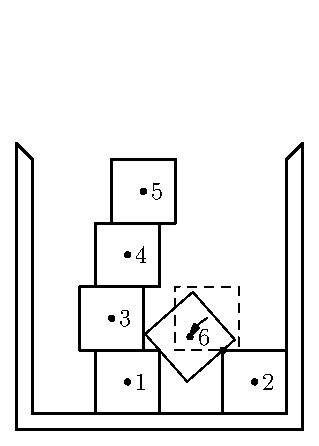
\includegraphics[height=\h]{btr-9}}%
\only<11>{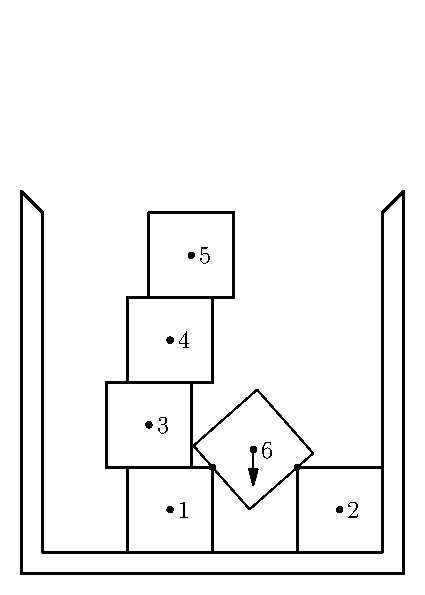
\includegraphics[height=\h]{btr-10}}%
\only<12>{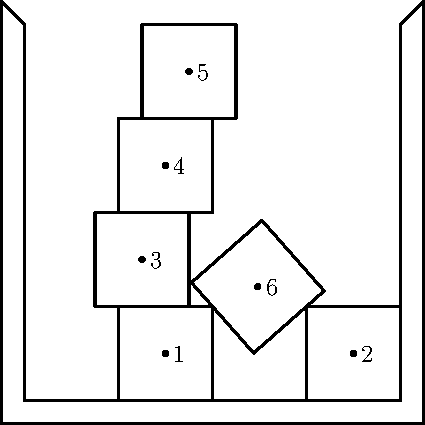
\includegraphics[height=\h]{btr-11}}
\end{block}
\end{frame}

\begin{frame}
\frametitle{References}
\printbibliography
\end{frame}

\end{document}
